\documentclass[stu,12pt,floatsintext]{apa7}

\usepackage[spanish,american]{babel}
\usepackage[utf8]{inputenc}
\usepackage[T1]{fontenc}
\usepackage{mathptmx}
\usepackage{csquotes}
\usepackage[style=apa,sortcites=true,sorting=nyt,backend=biber]{biblatex}
\DeclareLanguageMapping{american}{american-apa}
\addbibresource{bibliography.bib}
\usepackage{amsmath}
\usepackage{booktabs}
\usepackage{graphicx}

\title{Estimacion Experimental del Tamano Angular Aparente del Sol}
\shorttitle{Tamano Angular Solar}
\author{Camilo, Jean Lucca, Daniel}
\duedate{\today}
\affiliation{Universidad de Antioquia}
\course{Introduccion a la Astronomia Practica}
\professor{Docente del curso}

\abstract{Se estimo el tamano angular aparente del Sol mediante observaciones temporales de transito, usando la relacion $\theta = \omega t$ con $\omega = 15^\circ/\mathrm{h}$. Se analizaron 34 mediciones de tiempo con estadistica descriptiva, propagacion de incertidumbre e inferencia estadistica usando \texttt{scipy.stats}. La media observada fue $t=3.283\,\mathrm{min}$, equivalente a $\bar{\theta}=0.821^\circ$. Se obtuvo una incertidumbre instrumental de $\delta t=0.25\,\mathrm{min}$ y $\delta\theta=0.0625^\circ$. Las pruebas de normalidad (Shapiro-Wilk y D'Agostino-Pearson) rechazaron normalidad estricta, y una prueba t de una muestra detecto diferencia significativa frente al valor teorico de referencia $\theta_0\approx0.53^\circ$ ($p\approx1.05\times10^{-6}$, $d\approx1.02$). Se discuten posibles sesgos sistematicos asociados a la observacion visual y al cronometraje.}

\begin{document}
\maketitle

\section{Introduccion}
El tamano angular aparente de un astro puede estimarse a partir de su desplazamiento angular aparente en el cielo y del tiempo que tarda en recorrer una distancia angular conocida. Para este experimento se uso la relacion
\begin{equation}
\theta = \omega t,
\end{equation}
donde $\omega$ es la velocidad angular aparente del cielo y $t$ es el tiempo medido durante la observacion. En condiciones ideales, para el Sol se espera un valor aproximado de $\theta_0\approx0.53^\circ$ \parencite{portilla2009elementos}.

El objetivo de esta practica fue obtener una estimacion experimental de $\theta$, cuantificar su incertidumbre e interpretar la discrepancia con el valor teorico en terminos metodologicos.

\section{Metodo}
\subsection{Datos y variables}
Se utilizaron 34 mediciones de tiempo ($t$, en minutos) registradas en el archivo de datos del proyecto. Se adopto
\begin{equation}
\omega = 15^\circ/\mathrm{h} = 0.25^\circ/\mathrm{min}.
\end{equation}

Para la incertidumbre instrumental se considero
\begin{equation}
\delta t = 15\,\mathrm{s} = 0.25\,\mathrm{min}.
\end{equation}
Por propagacion lineal de errores para una variable:
\begin{equation}
\delta\theta = \left|\frac{\partial \theta}{\partial t}\right|\delta t = \omega\,\delta t = 0.0625^\circ.
\end{equation}
Este procedimiento de propagacion se enmarca en el tratamiento clasico de incertidumbres para funciones de una variable medible \parencite{baird1991experimentacion}.

\subsection{Analisis estadistico}
Se calcularon estadisticos descriptivos (media, mediana, desviacion estandar, error estandar, cuartiles e intervalo de confianza del 95\%). Para la inferencia se aplicaron pruebas de normalidad (Shapiro-Wilk y D'Agostino-Pearson) y una prueba t de una muestra contra el valor teorico de referencia. Tambien se reporto el tamano del efecto (Cohen's d). El procesamiento se realizo con \texttt{NumPy}, \texttt{pandas}, \texttt{SciPy}, \texttt{Matplotlib} y \texttt{Plotly} \parencite{harris2020array, mckinney2010data, virtanen2020scipy, hunter2007matplotlib, plotly2015}.

\section{Resultados}
\subsection{Estadistica descriptiva}
La Tabla~\ref{tab:descriptivos} resume los resultados principales.

\begin{table}[h!]
\caption{Resumen de estadistica descriptiva y propagacion de incertidumbre.}
\centering
\begin{tabular}{lr}
\toprule
Magnitud & Valor \\
\midrule
Numero de mediciones ($n$) & 34 \\
Media de $t$ [min] & 3.283 \\
Mediana de $t$ [min] & 2.941 \\
Desviacion estandar de $t$ [min] & 1.135 \\
Error estandar de $t$ [min] & 0.195 \\
IC 95\% de la media de $t$ [min] & [2.887, 3.679] \\
Media de $\theta$ [deg] & 0.821 \\
IC 95\% de la media de $\theta$ [deg] & [0.722, 0.920] \\
Incertidumbre instrumental $\delta t$ [min] & 0.250 \\
Incertidumbre propagada $\delta\theta$ [deg] & 0.0625 \\
\bottomrule
\end{tabular}
\label{tab:descriptivos}
\end{table}

Las graficas de serie de tiempo, histograma y valores de $\theta$ con barras de error se generaron en el cuaderno de analisis del proyecto y respaldan visualmente la dispersion observada.

\begin{figure}[h!]
\centering
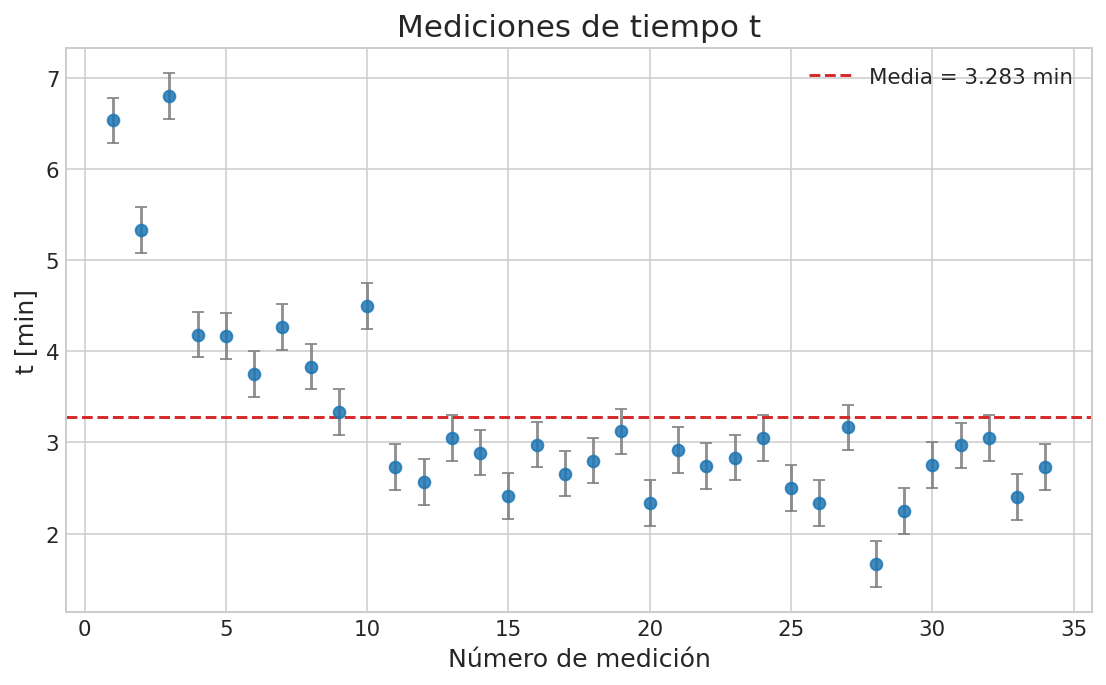
\includegraphics[width=0.95\textwidth]{MedicionesDeTiempo_t.png}
\caption{Serie temporal de las mediciones del tiempo de transito $t$ (min) para las 34 observaciones. Se aprecia variabilidad inter-observacion y presencia de valores altos aislados.}
\label{fig:serie_t}
\end{figure}

\begin{figure}[h!]
\centering
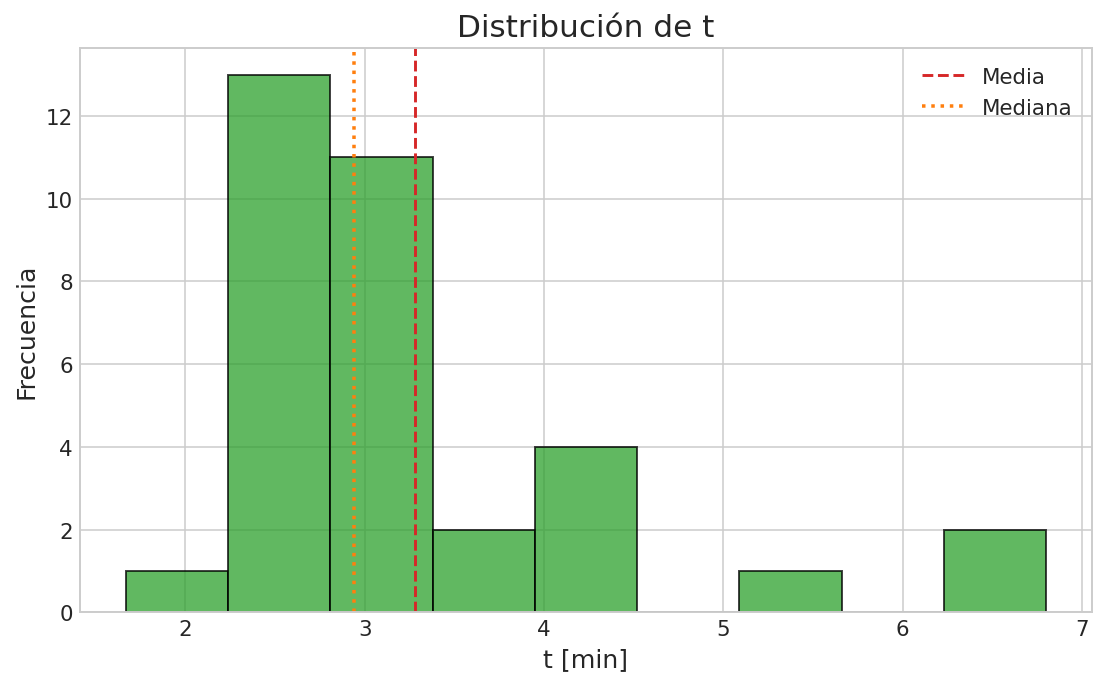
\includegraphics[width=0.95\textwidth]{DistribucionDe_t.png}
\caption{Distribucion empirica de $t$ mediante histograma y curva de densidad. La forma asimetrica es consistente con el rechazo de normalidad en las pruebas inferenciales.}
\label{fig:hist_t}
\end{figure}

\begin{figure}[h!]
\centering
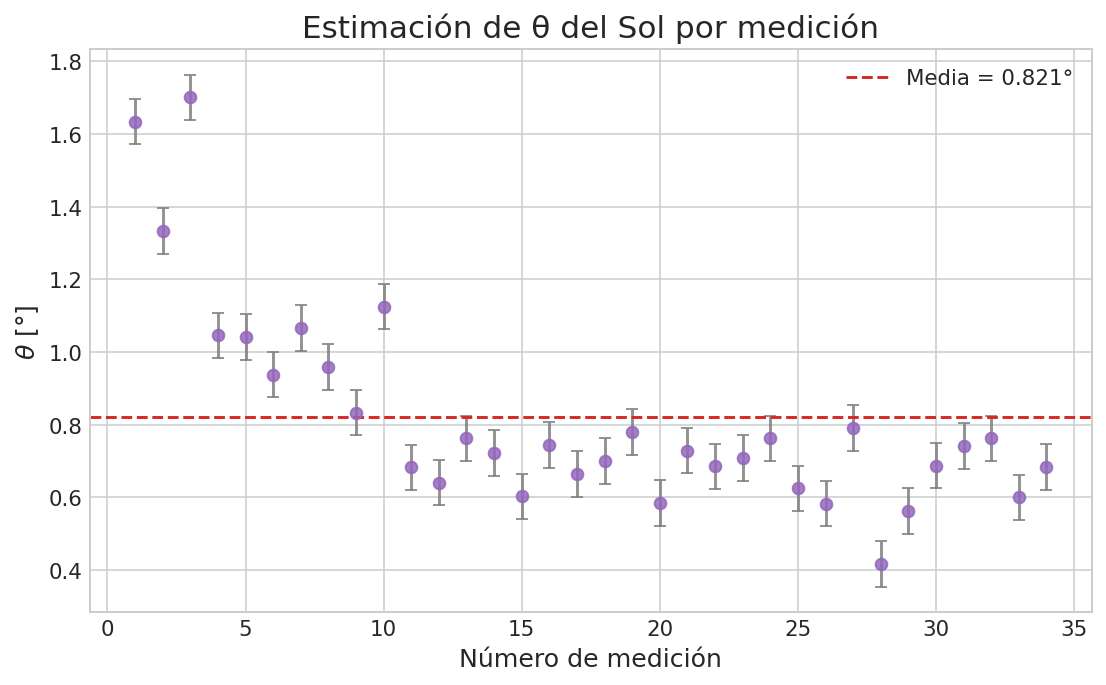
\includegraphics[width=0.95\textwidth]{EstimacionDe_theta.png}
\caption{Estimaciones individuales de $\theta$ con barra de error instrumental constante ($\pm 0.0625^\circ$) y linea de referencia teorica para el Sol.}
\label{fig:theta_err}
\end{figure}

\subsection{Estadistica inferencial}
Los resultados inferenciales se presentan en la Tabla~\ref{tab:inferencial}.

\begin{table}[h!]
\caption{Pruebas inferenciales con \texttt{scipy.stats}.}
\centering
\begin{tabular}{lrr}
\toprule
Prueba & Estadistico & p-valor \\
\midrule
Shapiro-Wilk sobre $t$ & 0.810 & 0.000041 \\
D'Agostino-Pearson sobre $t$ & 20.018 & 0.000045 \\
t-test 1 muestra ($\theta$ vs. $\theta_0=0.53^\circ$) & 5.972 & 0.000001 \\
\bottomrule
\end{tabular}
\label{tab:inferencial}
\end{table}

Ambas pruebas de normalidad rechazan normalidad estricta para $t$ al nivel $\alpha=0.05$. Aun asi, la prueba t de una muestra muestra que la media experimental difiere significativamente del valor de referencia teorico reportado para el Sol \parencite{portilla2009elementos}. El tamano del efecto fue grande ($d\approx1.024$).

\section{Discusion}
El valor medio estimado $\bar{\theta}=0.821^\circ$ supera el valor solar tipico de referencia ($\sim0.53^\circ$). Esta discrepancia es consistente con la naturaleza del procedimiento: la medicion visual del borde solar y el cronometraje manual introducen sesgos sistematicos y variabilidad adicional. Entre las fuentes de error plausibles estan el tiempo de reaccion del observador, la dificultad de definir el inicio y fin del evento observado, y condiciones atmosfericas locales.

La significancia estadistica encontrada no debe interpretarse como fracaso experimental, sino como evidencia de que, bajo las condiciones de campo empleadas, la estimacion contiene un componente sistematico relevante. En este contexto, el experimento cumple su objetivo formativo: conectar modelo fisico, propagacion de incertidumbre y analisis inferencial aplicado a datos reales.

\section{Conclusiones}
Se logro una estimacion experimental del tamano angular aparente del Sol y se implemento un flujo de analisis reproducible. Los resultados muestran:
\begin{itemize}
    \item estimacion media de $\theta$ mayor que el valor teorico de referencia;
    \item incertidumbre instrumental cuantificada y propagada de forma explicita;
    \item diferencia estadisticamente significativa frente a la referencia teorica;
    \item evidencia de sesgos sistematicos asociados al metodo de observacion.
\end{itemize}

Como mejora metodologica, se recomienda aumentar repeticiones por sesion, estandarizar criterios de inicio/fin de cronometraje, y usar registros asistidos (video o sensores) para reducir sesgo humano.

\printbibliography

\end{document}
